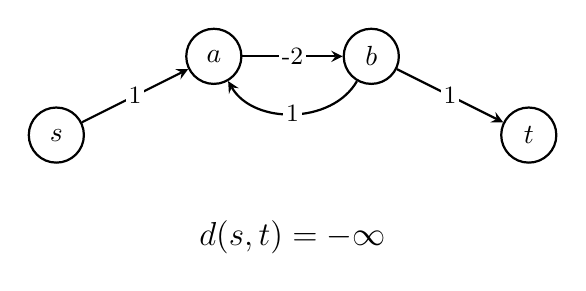
\begin{tikzpicture}[
    scale=1,
    vertex/.style={draw, circle, thick, minimum size=7mm, inner sep=0pt},
    diredge/.style={->, thick, >=stealth},
    weight/.style={fill=white, inner sep=1pt, font=\small}
]

\node[vertex] (s) at (0,0) {$s$};
\node[vertex] (a) at (2,1) {$a$};
\node[vertex] (b) at (4,1) {$b$};
\node[vertex] (t) at (6,0) {$t$};

\draw[diredge] (s) -- node[weight] {1} (a);
\draw[diredge] (a) -- node[weight] {-2} (b);
\draw[diredge] (b) to[bend left=60] node[weight] {1} (a);
\draw[diredge] (b) -- node[weight] {1} (t);

\node[align=center] at (3,-1.3) {\large $d(s,t)=-\infty$};

\end{tikzpicture}